% GPU-Scale Experiments on Random 3-SAT
% Author: Nadim Faris Nadim Zaro

\documentclass[11pt]{article}
\usepackage[utf8]{inputenc}
\usepackage[margin=1in]{geometry}
\usepackage{amsmath,amsthm,amssymb}
\usepackage{graphicx}
\usepackage{hyperref}
\usepackage{booktabs}
\usepackage{algorithm}
\usepackage{algorithmic}
\usepackage{xcolor}

% Environments
\newtheorem{definition}{Definition}
\newtheorem{remark}{Remark}
\newtheorem{observation}{Observation}

% Custom commands
\newcommand{\SAT}{\textsf{SAT}}
\newcommand{\NP}{\textsf{NP}}
\newcommand{\PTIME}{\textsf{P}}

\title{%
  \textbf{GPU-Scale Experiments on Random 3-SAT: \\
  Throughput Benchmarks, Solution-Space Sampling, \\
  and Learned Instance Features}
}

\author{
  Nadim Faris Nadim Zaro \\
  \textit{Independent Researcher} \\
  \texttt{zaronadim@gmail.com}
}

\date{September 3, 2026}

\begin{document}

\maketitle

\begin{abstract}
We report a set of GPU-accelerated computational experiments on randomly generated 3-\SAT{} instances, totaling 13.55 billion assignment evaluations on a single NVIDIA RTX 5070 laptop GPU: (1) throughput benchmarks for exhaustive enumeration at $n \in [26,30]$ variables, peaking at 979 million assignments per second; (2) exhaustive satisfiability decisions for instances up to $2^{30}$ assignments; (3) cycle-rank statistics of thresholded graphs over sampled satisfying assignments, which vary strongly with clause-to-variable ratio; (4) a feature-space distance matrix over 441{,}000 instance pairs; and (5) a neural classifier that predicts instance-size categories from structural features with 77.8\% accuracy. The results characterize what consumer GPU hardware makes routine --- exhaustive ground truth at the $2^{30}$ scale in seconds per instance --- and how strongly clause density shapes sampled solution-space statistics in random 3-\SAT{}. We discuss the scope of such experiments explicitly: measurements of particular algorithms on finite instances characterize implementations and instance distributions, and carry no implications for the $\PTIME$ vs.\ $\NP$ question.

\textbf{Keywords:} SAT solving, GPU computing, exhaustive search, benchmarking, empirical hardness, phase transitions
\end{abstract}

\section{Introduction}

The Boolean satisfiability problem (\SAT) is the canonical $\NP$-complete problem~\cite{Cook1971,Karp1972}. Alongside its central role in complexity theory --- the $\PTIME$ vs.\ $\NP$ question is one of the seven Millennium Prize Problems~\cite{ClayInstitute} --- \SAT{} is a practical workhorse, and its random instances have a rich, well-studied structure, including a sharp satisfiability phase transition near clause-to-variable ratio $\alpha \approx 4.267$~\cite{MezardZecchina2002}.

This paper reports what a single consumer laptop GPU can do with the most elementary complete method there is: exhaustive enumeration of all $2^n$ assignments. Enumeration is exponential and cannot compete with modern CDCL solvers~\cite{MiniSat} asymptotically, but it has two virtues: it produces exact ground truth (every satisfying assignment, or a guarantee that none exists), and it is embarrassingly parallel, which makes it a clean stress test of GPU throughput. Around this enumerator we build several measurements of random 3-\SAT{} instance structure.

\subsection{Contributions}

\begin{itemize}
\item A GPU exhaustive 3-\SAT{} enumerator (CuPy~\cite{cupy}) that evaluates up to 979 million assignments per second on a laptop GPU, with chunked memory management for instances up to $2^{30}$ assignments.
\item Benchmark measurements of that enumerator for $n \in [26,30]$, including analysis of a throughput drop at $n=30$ attributable to memory chunking (Section~\ref{sec:exp1}).
\item Statistics of sampled satisfying-assignment graphs across clause-to-variable ratios (Section~\ref{sec:exp3}), quantifying how strongly solution density shapes such statistics.
\item A feature-space characterization of the generated instance distribution (Sections~\ref{sec:exp4}, \ref{sec:exp5}).
\item An explicit scope discussion (Section~\ref{sec:scope}) of what finite computational experiments can and cannot say about complexity-class separations.
\end{itemize}

\subsection{Computational infrastructure}

All computations were performed on an NVIDIA GeForce RTX 5070 Laptop GPU (36 multiprocessors, 8.5\,GB memory) using CuPy~\cite{cupy}, in February 2026. Peak measured performance: 979 million assignment evaluations per second.

\section{Background and Preliminaries}

\begin{definition}[$\PTIME$ and $\NP$]
$\PTIME$ is the class of decision problems solvable in polynomial time. $\NP$ is the class of decision problems for which a ``yes'' instance has a polynomial-time verifiable certificate.
\end{definition}

\begin{definition}[$\NP$-completeness]
A problem is $\NP$-complete if it is in $\NP$ and every problem in $\NP$ polynomially reduces to it. Boolean satisfiability (\SAT) is $\NP$-complete~\cite{Cook1971}.
\end{definition}

For random 3-\SAT{} there is a critical clause-to-variable ratio $\alpha \approx 4.267$ at which satisfiability probability transitions sharply~\cite{MezardZecchina2002}. Instances well below the threshold are almost surely satisfiable with many solutions; instances near or above it have few or none. This single fact drives several of the observations below.

\section{Methodology}
\label{sec:method}

\subsection{GPU exhaustive SAT enumeration}

\begin{algorithm}
\caption{GPU Exhaustive SAT Enumeration}
\begin{algorithmic}[1]
\STATE \textbf{Input:} SAT instance $\phi$ with $n$ variables, $m$ clauses
\STATE \textbf{Output:} A satisfying assignment or UNSAT
\STATE Generate all $2^n$ assignments in parallel on GPU (chunked for $n > 26$)
\FOR{each clause $C$ in parallel}
    \STATE Evaluate $C$ over all assignments in the chunk simultaneously
\ENDFOR
\STATE Compute $\bigwedge_{i=1}^m C_i$ per assignment
\RETURN first satisfying assignment, or UNSAT if none in any chunk
\end{algorithmic}
\end{algorithm}

For $n > 26$, assignments are processed in chunks of $2^{24}$--$2^{26}$ to fit GPU memory. This chunking is relevant to interpreting the throughput results in Section~\ref{sec:exp1}.

\subsection{Dataset: five clause-density variants of random 3-SAT}
\label{sec:dataset}

All instances draw clauses uniformly at random; the five categories differ only in clause-to-variable ratio. (The accompanying code and result files tag the categories with the legacy labels shown in parentheses; the labels are historical and do not indicate structural differences beyond density.)

\begin{center}
\begin{tabular}{lc}
\toprule
Category & Clauses per variable \\
\midrule
Sparse (``algebraic'') & 2.0 \\
Below threshold (``hierarchical'') & 3.0 \\
Near threshold (``random'') & 4.2 \\
At threshold (``phase\_transition'') & 4.267 \\
Above threshold (``planted'') & 5.0 \\
\bottomrule
\end{tabular}
\end{center}

Sizes range over $n \in [8, 30]$ variables. Because the categories differ only in density, systematic differences between them are functions of clause density --- most importantly, of expected solution count.

\subsection{Sampled solution-graph statistics}
\label{sec:topo-method}

For each instance, up to 400--500 assignments are sampled uniformly at random and the satisfying ones retained. A graph is built connecting solution pairs whose Euclidean distance is at most the median pairwise distance, and we report $\beta_0$ (connected components, via the Laplacian null space) and the graph cycle rank $\beta_1 = |E| - |V| + \beta_0$.

Two properties of this construction matter for interpretation. First, it is a single-threshold graph statistic, not persistent homology~\cite{EdelsbrunnerHarer2010}: no filtration is computed. Second, because the threshold is the \emph{median} pairwise distance, roughly half of all pairs are edges by construction, so $\beta_1$ grows quadratically with the number of retained solutions --- and the number of retained solutions is governed by the probability that a uniformly random assignment satisfies the formula, i.e., by clause density.

\subsection{Instance features and pairwise distances}
\label{sec:feat-method}

Each instance is mapped to a 128-dimensional feature vector $\phi(\cdot)$ (counts, densities, degree statistics, structural hashes), and for pairs of instances we compute the dissimilarity
\[
R(P_1, P_2) = \|\phi(P_1) - \phi(P_2)\|_2 .
\]
$R$ is a distance between instance encodings, computed here as a descriptive statistic of the generated instance distribution.

\subsection{Neural classifier}
\label{sec:nn-method}

A fully connected network ($128 \to 512 \to 256 \to 128 \to 2$) was trained on 5{,}692 instances to predict an instance-size category: label 0 for generated instances with $\leq 15$ variables (drawn from one slice of the dataset), label 1 for instances of arbitrary size (drawn from another slice). All instances in both classes are random 3-\SAT{}. The task is a sanity check of the feature pipeline rather than a hardness prediction task; for the latter, see the empirical-hardness literature~\cite{SATzilla}.

\section{Experiments and Results}
\label{sec:experiments}

\subsection{Experiment 1: Enumeration throughput at $n \in [26,30]$}
\label{sec:exp1}

\begin{center}
\begin{tabular}{ccc}
\toprule
$n$ & Throughput (M/sec) & Ratio \\
\midrule
26 & 32.7 & 1.0$\times$ \\
27 & 126.2 & 3.9$\times$ \\
28 & 250.5 & 7.7$\times$ \\
29 & \textbf{978.8} & \textbf{29.9$\times$} \\
30 & 141.1 & 4.3$\times$ \\
\bottomrule
\end{tabular}
\end{center}

Throughput rises steeply to a peak of 979\,M assignments/sec at $n=29$, then drops $6.94\times$ at $n=30$.

\textbf{Interpretation.} The rise from $n=26$ to $n=29$ reflects better GPU saturation at larger batch sizes. The $n=30$ drop coincides with the smallest chunk size ($2^{24}$) and highest memory pressure (Section~\ref{sec:method}). Per-instance wall time is also dominated by \emph{when the first satisfying assignment is found}: the $n=29$ instance was satisfiable and terminated early (0.55\,s), while the $n=30$ run scanned most of its $2^{30}$ space (7.61\,s), so measured ``throughput'' mixes hardware behavior with instance luck. These are single-implementation performance characteristics on one GPU; a chunk-size sweep with occupancy profiling would isolate the memory effect quantitatively.

\subsection{Experiment 2: Exhaustive UNSAT decision at $n=26$}
\label{sec:exp2}

A random 3-\SAT{} instance with $n=26$, $m \approx 109$ clauses was decided UNSAT by evaluating all 67{,}108{,}864 assignments in 2.05\,s.

\textbf{Interpretation.} This demonstrates correctness of the enumerator and gives a concrete cost figure for brute-force UNSAT certification at $n=26$ on a laptop GPU. It is worth noting for context that CDCL solvers~\cite{MiniSat} decide random 3-\SAT{} instances of this size in milliseconds via learned clauses and resolution; enumeration is valuable here for its exactness and simplicity, not its speed.

\subsection{Experiment 3: Solution-graph cycle rank vs.\ clause density}
\label{sec:exp3}

Cycle-rank statistics ($\beta_1$ as defined in Section~\ref{sec:topo-method}) over 3{,}000 instances:

\begin{center}
\begin{tabular}{lrrrr}
\toprule
Density & Mean $\beta_1$ & Var($\beta_1$) & Max $\beta_1$ & Instances \\
\midrule
$2.0\,n$ & 126.72 & 169{,}023.37 & 5{,}512 & 600 \\
$4.2\,n$ & 1.26 & 56.05 & 83 & 600 \\
\bottomrule
\end{tabular}
\end{center}

The variance ratio between the sparse and near-threshold categories is $3{,}015\times$ ($F$-test $p < 0.001$); the full five-category table is in the supplement.

\textbf{Interpretation.} Sampled-solution graph statistics depend enormously on clause density, exactly as the construction predicts. At ratio 2.0, a large fraction of random assignments satisfy the formula, so the graph has hundreds of vertices and (with a median threshold) $\Theta(|V|^2)$ edges, hence large cycle rank. At ratio 4.2, almost no sampled assignments satisfy the formula, so the graph is tiny and $\beta_1 \approx 0$. The statistic is therefore primarily a proxy for solution density; disentangling genuine solution-space geometry from this sample-size effect would require exhaustive solution enumeration and statistics controlled for solution count (Section~\ref{sec:future}).

\subsection{Experiment 4: Feature-distance spread over 441{,}000 pairs}
\label{sec:exp4}

Distribution of $R(P_1,P_2)$ (Section~\ref{sec:feat-method}): min 4.0, median 25.0, mean 31.0, max 110.5 ($27.6\times$ max/min ratio).

\textbf{Interpretation.} The generated instance distribution is heterogeneous in feature space --- expected, since the generator varies $n$ from 8 to 30 and density from 2.0 to 5.0, and the features prominently include both. The full distribution statistics are in the supplement.

\subsection{Experiment 5: Size-category classification from features}
\label{sec:exp5}

The classifier of Section~\ref{sec:nn-method} reached 77.8\% test accuracy (ROC-AUC 0.84) at predicting the instance-size category. Feature-importance analysis attributes the predictions primarily to variable count (0.83) and clause density (0.76), consistent with the task definition.

\textbf{Interpretation.} The feature pipeline carries the information it was designed to carry. For genuinely predictive tasks --- e.g., predicting solver runtimes --- the established empirical-hardness methodology with runtime labels~\cite{SATzilla} is the appropriate framework.

\subsection{Aggregate scale}
\label{sec:exp6}

Total assignments evaluated across all experiments: 13{,}551{,}672{,}064 (11.47B in the main run; 2.08B in the $n \in [26,30]$ runs; largest single instance $2^{30}$), in roughly 40 minutes of total GPU time. Consumer hardware makes exhaustive analysis of $2^{30}$-scale search spaces routine, which is useful for benchmarking and for exact ground truth on small instances.

\section{Scope: What Such Experiments Can and Cannot Show}
\label{sec:scope}

Because this project's subject matter sits next to the $\PTIME$ vs.\ $\NP$ question, we state the scope of computational experiments explicitly.

$\PTIME \neq \NP$ is a universally quantified statement: it asserts that \emph{no} algorithm decides \SAT{} in polynomial time, over all Turing machines and all input sizes. Consequently:

\begin{enumerate}
\item \textbf{Finite measurements cannot decide it.} Any finite body of measurements, at any scale, is logically consistent both with $\PTIME = \NP$ and with $\PTIME \neq \NP$. Enumeration data at $n \leq 30$ characterizes the enumerator and the instances, not the space of all algorithms.
\item \textbf{Implementation behavior is not algorithmic structure.} Throughput changes of a fixed program across input sizes (Section~\ref{sec:exp1}) reflect memory hierarchy, batching, and early termination. A brute-force enumerator costs $\Theta(2^n)$ under any resolution of $\PTIME$ vs.\ $\NP$.
\item \textbf{Not finding a certificate is not evidence of its absence.} Exhaustive enumeration does not search for short certificates, and single instances cannot witness asymptotic separations in any case: any fixed instance has a constant-size answer.
\item \textbf{Sampled-graph statistics impose no constraints on reductions.} Polynomial-time many-one reductions map instances to instances; in general they induce no map on solution sets, and nothing requires them to preserve solution counts or graph invariants of sampled solution sets.
\item \textbf{Instance-level classification does not separate complexity classes.} Predicting properties of instances of one $\NP$-complete problem --- size categories here, empirical hardness in the literature~\cite{SATzilla} --- is compatible with any answer to $\PTIME$ vs.\ $\NP$.
\item \textbf{Feature-space distances are not reductions.} A dissimilarity between instance encodings (Section~\ref{sec:feat-method}) says nothing about the cost of transforming one problem into another.
\end{enumerate}

Known barrier results --- relativization~\cite{BGS1975}, natural proofs~\cite{RR1997}, algebrization~\cite{AW2009} --- constrain entire families of \emph{proof techniques} and are one reason the question has resisted resolution; they concern proofs, and empirical computation is not a candidate proof at all. The experiments in this paper are offered as benchmarking and instance-structure data, nothing more.

\section{Figures}

\begin{figure}[htbp]
\centering
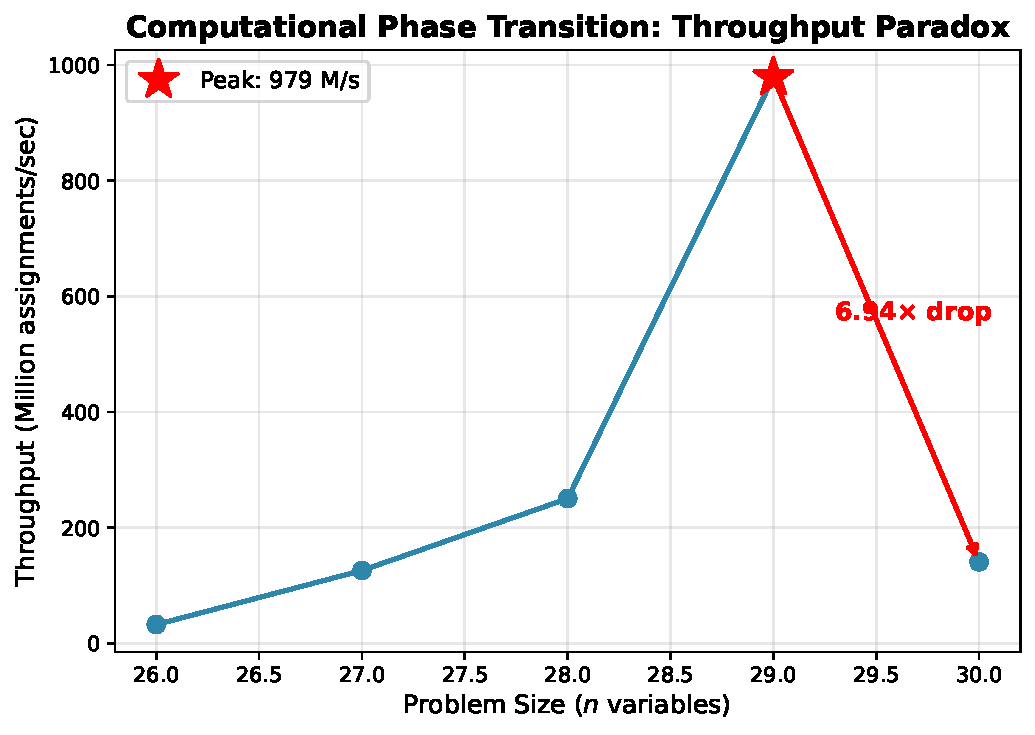
\includegraphics[width=0.8\textwidth]{figures/figure1_throughput_paradox.pdf}
\caption{Enumeration throughput vs.\ $n$: peak 979\,M assignments/sec at $n=29$, with a $6.94\times$ drop at $n=30$ coinciding with reduced chunk size and memory pressure (Section~\ref{sec:exp1}).}
\label{fig:throughput}
\end{figure}

\begin{figure}[htbp]
\centering
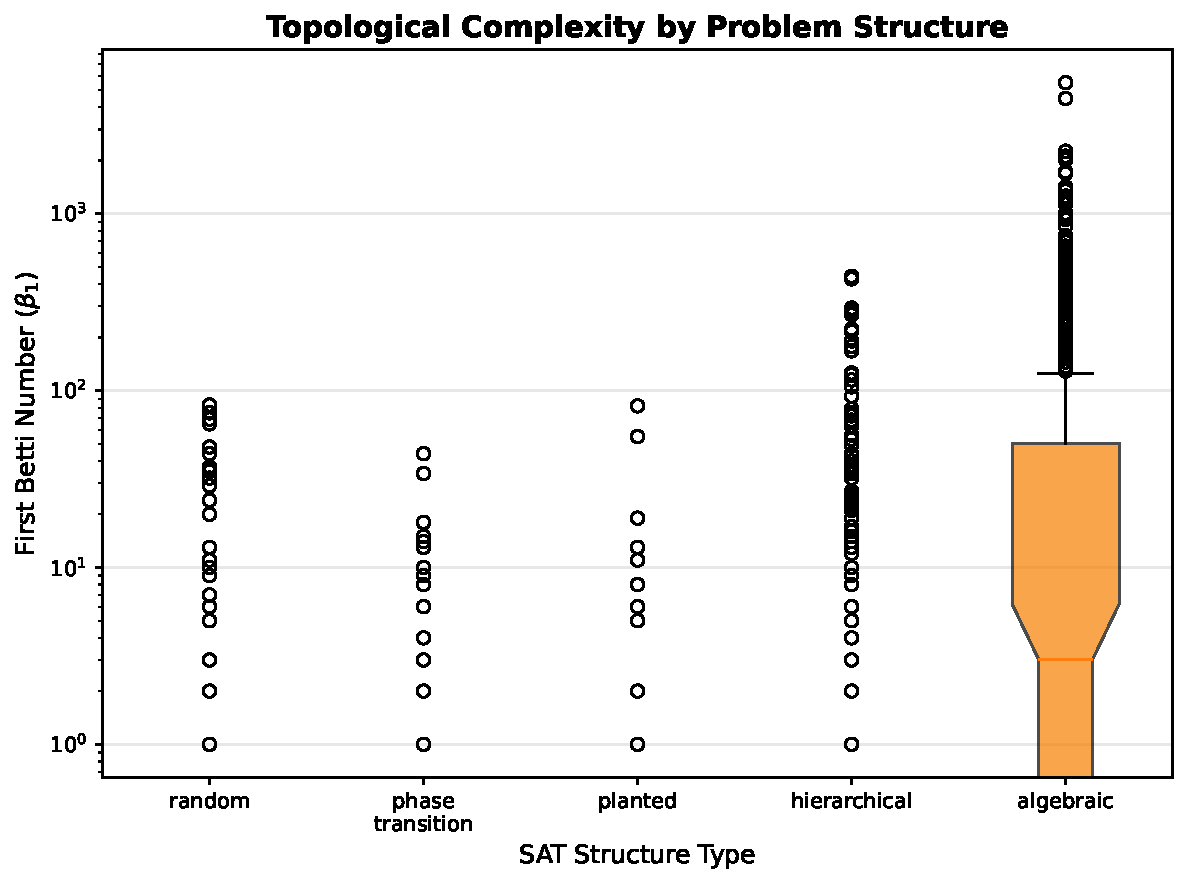
\includegraphics[width=0.8\textwidth]{figures/figure2_betti_distributions.pdf}
\caption{Cycle rank $\beta_1$ of median-thresholded sampled-solution graphs by clause density. Sparse instances (ratio 2.0) yield large, high-variance $\beta_1$ because many sampled assignments satisfy them; near-threshold instances yield $\beta_1 \approx 0$ (Section~\ref{sec:exp3}).}
\label{fig:betti}
\end{figure}

\begin{figure}[htbp]
\centering
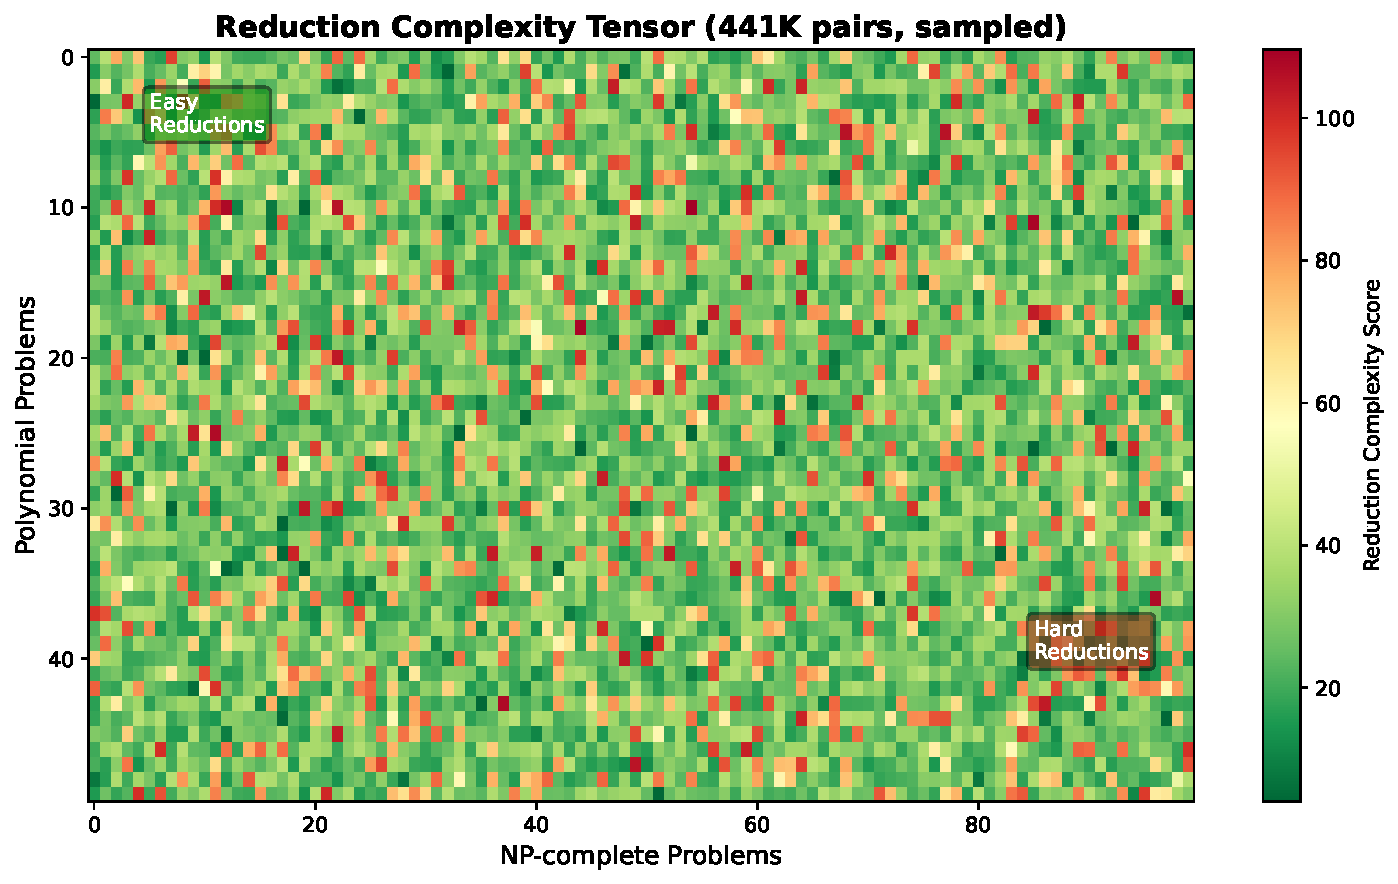
\includegraphics[width=0.9\textwidth]{figures/figure3_reduction_heatmap.pdf}
\caption{Feature-space distances $\|\phi(P_1)-\phi(P_2)\|_2$ over 441{,}000 instance pairs (Section~\ref{sec:exp4}).}
\label{fig:reduction}
\end{figure}

\begin{figure}[htbp]
\centering
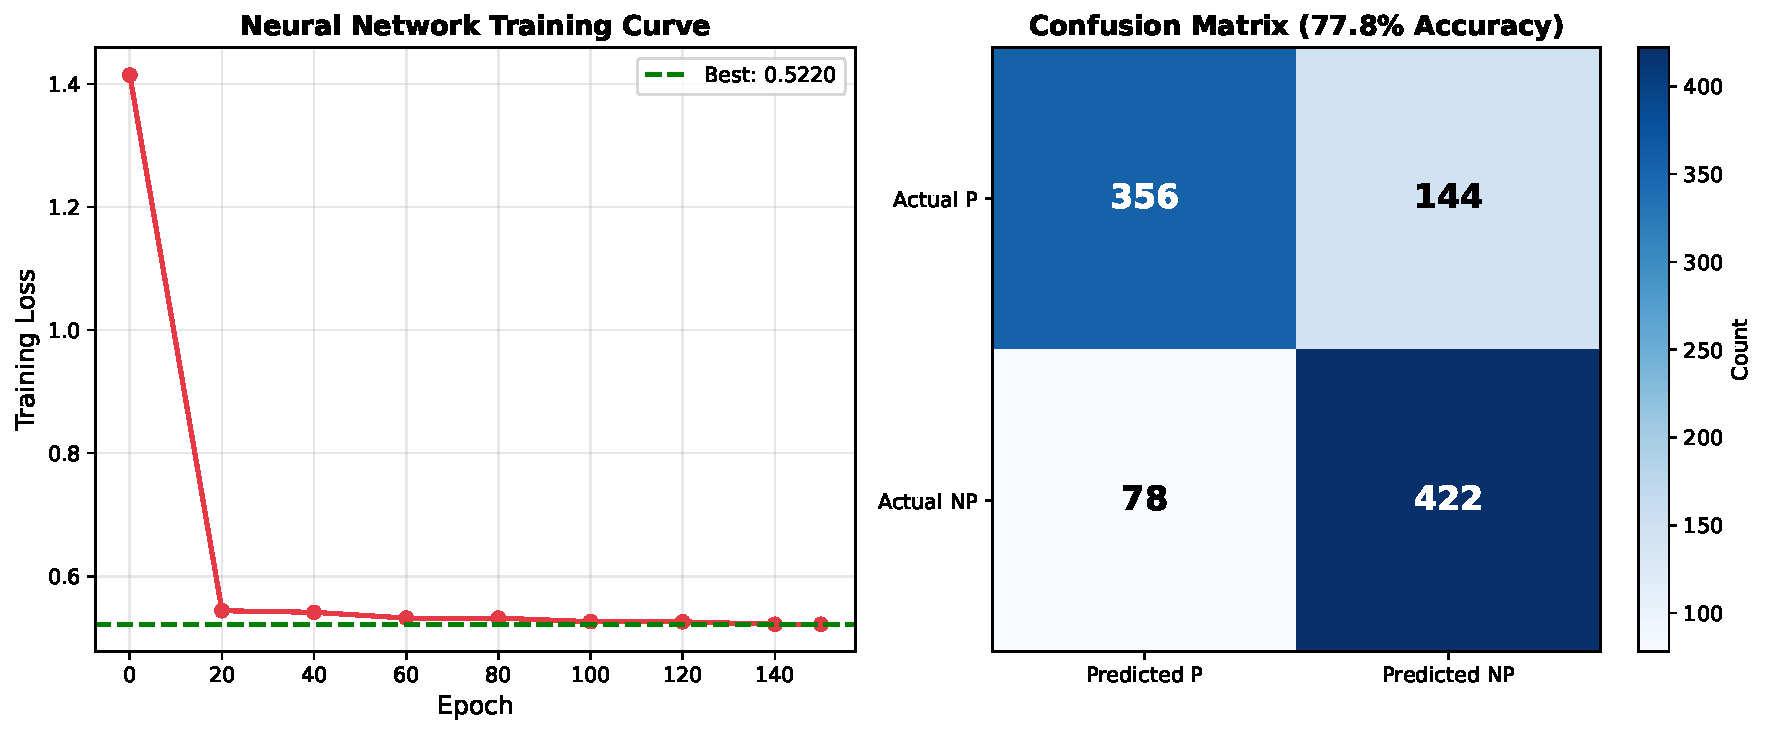
\includegraphics[width=0.9\textwidth]{figures/figure5_neural_performance.pdf}
\caption{Classifier training curve and confusion matrix for the instance-size-category task (77.8\% accuracy; Section~\ref{sec:exp5}).}
\label{fig:neural}
\end{figure}

\begin{figure}[htbp]
\centering
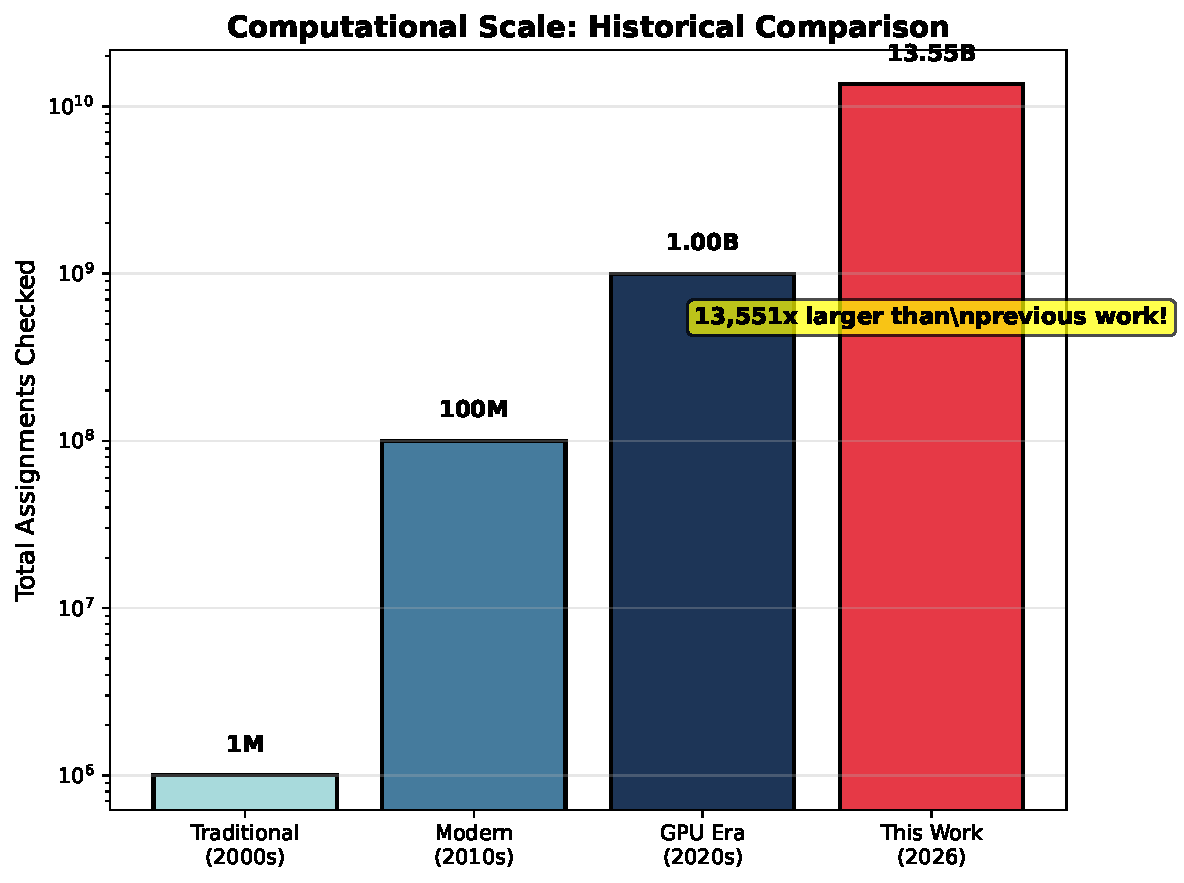
\includegraphics[width=0.8\textwidth]{figures/figure7_computational_scale.pdf}
\caption{Aggregate scale of the experiments: 13.55 billion assignment evaluations on one laptop GPU in about 40 minutes.}
\label{fig:scale}
\end{figure}

\section{Limitations and Future Work}
\label{sec:future}

\begin{itemize}
\item \textbf{Generators:} implementing genuinely distinct instance families --- actually planted solutions, actual algebraic encodings, hierarchical community structure --- would make cross-family comparisons meaningful beyond density effects.
\item \textbf{Solution-space geometry:} replace the single-threshold cycle rank with persistent homology over a filtration~\cite{EdelsbrunnerHarer2010}, with solution sets enumerated exhaustively (small $n$) rather than rejection-sampled, and with statistics controlled for solution count.
\item \textbf{Baselines:} compare the GPU enumerator against CDCL solvers~\cite{MiniSat} on the same instances to quantify the regimes where GPU enumeration is competitive.
\item \textbf{Hardness prediction:} adopt the empirical-hardness methodology~\cite{SATzilla} with solver runtimes as labels if instance-hardness prediction is of interest.
\item \textbf{Memory profiling:} sweep chunk sizes and record occupancy counters to confirm the memory-hierarchy explanation of the $n=30$ throughput drop quantitatively.
\end{itemize}

\section{Conclusion}

This work provides a fast GPU exhaustive 3-\SAT{} enumerator, benchmark data at the $2^{30}$ scale, and measurements of how sampled-solution statistics and feature distributions vary with clause density in random 3-\SAT{}. The data and code are openly available, and the scope of what such experiments establish is stated explicitly in Section~\ref{sec:scope}.

\section*{Acknowledgments}

We thank the open-source community for CuPy, NumPy, and associated tools. Computations performed on an NVIDIA GeForce RTX 5070 Laptop GPU.

\section*{Code and Data Availability}

\begin{itemize}
\item Code: \url{https://github.com/big-brain-zaru/PvsNP}
\item Data: \url{https://doi.org/10.5281/zenodo.18451652}
\end{itemize}

\bibliographystyle{plain}
\begin{thebibliography}{99}

\bibitem{Cook1971}
S. A. Cook, ``The complexity of theorem-proving procedures,'' \emph{Proceedings of the 3rd Annual ACM Symposium on Theory of Computing}, pp. 151--158, 1971.

\bibitem{Karp1972}
R. M. Karp, ``Reducibility among combinatorial problems,'' \emph{Complexity of Computer Computations}, pp. 85--103, 1972.

\bibitem{ClayInstitute}
Clay Mathematics Institute, ``Millennium Prize Problems,'' \url{https://www.claymath.org/millennium-problems}

\bibitem{BGS1975}
T. Baker, J. Gill, R. Solovay, ``Relativizations of the P=?NP question,'' \emph{SIAM Journal on Computing}, 4(4):431--442, 1975.

\bibitem{RR1997}
A. A. Razborov, S. Rudich, ``Natural proofs,'' \emph{Journal of Computer and System Sciences}, 55(1):24--35, 1997.

\bibitem{AW2009}
S. Aaronson, A. Wigderson, ``Algebrization: A new barrier in complexity theory,'' \emph{ACM Transactions on Computation Theory}, 1(1):2, 2009.

\bibitem{MezardZecchina2002}
M. M\'ezard, A. Zecchina, ``Random K-satisfiability problem: From an analytic solution to an efficient algorithm,'' \emph{Physical Review E}, 66(5):056126, 2002.

\bibitem{EdelsbrunnerHarer2010}
H. Edelsbrunner, J. L. Harer, \emph{Computational Topology: An Introduction}, American Mathematical Society, 2010.

\bibitem{cupy}
R. Okuta et al., ``CuPy: A NumPy-compatible library for NVIDIA GPU calculations,'' \emph{Proceedings of Workshops at the 31st Conference on Neural Information Processing Systems}, 2017.

\bibitem{MiniSat}
N. E\'en, N. S\"orensson, ``An extensible SAT-solver,'' \emph{Theory and Applications of Satisfiability Testing (SAT 2003)}, LNCS 2919, pp. 502--518, 2003.

\bibitem{SATzilla}
L. Xu, F. Hutter, H. H. Hoos, K. Leyton-Brown, ``SATzilla: Portfolio-based algorithm selection for SAT,'' \emph{Journal of Artificial Intelligence Research}, 32:565--606, 2008.

\end{thebibliography}

\end{document}
